
\documentclass{article}
\usepackage[utf8]{inputenc}
\usepackage{algorithm2e}
\usepackage{amsmath}
\usepackage{graphicx}

\title{OCEL Feature Extraction Documentation}
\date{November 2021 - ??? 2022}

\begin{document}

\maketitle

\tableofcontents
\pagebreak

\section{Document Format}
The structure section will go over all the structures that are created in order for many of the feature extraction methods to function. Each structure will have information on input, context behind the structure and a sample image to demonstrate the output on a basic example.

The Feature sections go over feature extraction methods explored throughout the thesis on the topic. All features are aimed at being very general, applicable to any input ocel log. The descriptions will include the input, structures used, output, context and, if required, a very small basic visualization based on the examples that are found in the structures section. 
)

\section{Example OCEL}
The following log was taken from ... and will be used for the majority of examples in this document. Of course this log is very basic and will therefore not cover all edge cases that can occur in ocel logs. However, using the log, I hope to show the intuition of all structures and feature extraction methods.

\begin{figure}[h]
	\centering
	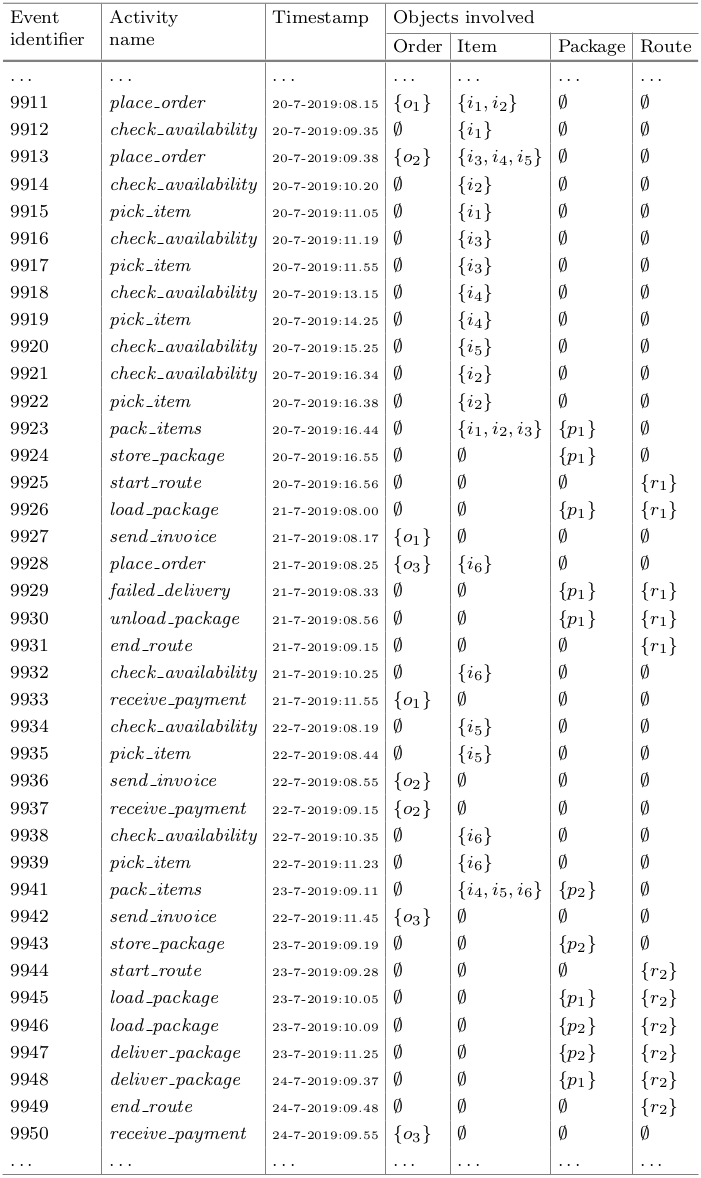
\includegraphics[scale=0.2496]{images/ocel.png}
	\caption{Simple example log}
	\label{fig:log}
\end{figure}

\section{Structures}
\subsection{Object-Based}
\subsubsection{Object Interaction Graph}
\textbf{Description -} This \emph{undirected} graph simply places all objects on the graph as \emph{nodes} and assigns \emph{edges} based on whether an object interacted in the same event as the other.\\

\noindent \textbf{Context -} The goal of this graph is to provide a base graph that allows relationships between objects to be explored.
\\

\noindent\textbf{Strengths}
\begin{enumerate}
	\item Very simple
	\item Allows for initial relationships between all objects
\end{enumerate}

\noindent\textbf{limitations}
\begin{enumerate}
	\item Very high number of edges
	\item An object that interacts a lot with a target object is displayed the same as an object with very few interaction
\end{enumerate}

\noindent\textbf{Visual example}
\begin{figure}[h]
	\centering
	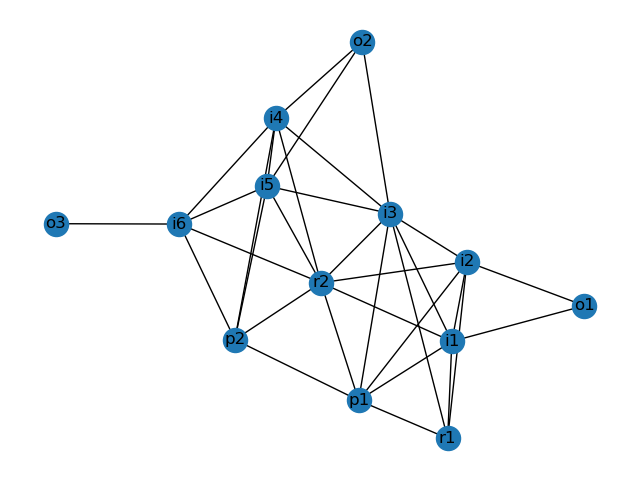
\includegraphics[scale=0.5]{images/object-graph.png}
	\caption{Example of an Object Interaction Graph}
	\label{fig:object-graph}
\end{figure}


\subsubsection{Object Descendant Graph}
\textbf{Description -} This \emph{directed} graph places all objects on the graph as \emph{nodes} and assigns \emph{edges} based on whether an source object participated in the event where the target object participated in its first event. Note that this also means that objects that were created in the same event are descendants of each other.\\

\noindent \textbf{Context -} The goal of this graph is to take advantage of the time dimension in order to separate objects from each other. This helps greatly reduce the degree of each of the nodes.
\\

\noindent\textbf{Strengths}
\begin{enumerate}
	\item More focussed graph on objects that are related by the time dimension.
	\item Direction adds ability to easily segment further (via connectedness) and find independence between objects.
	\item Allows for disconnected subgraphs
\end{enumerate}

\noindent\textbf{limitations}
\begin{enumerate}
	\item Ignores object relationships related to frequency of interaction with each other.
	\item Can cause many objects to have no edges.
	\item General objects (eg. SYSTEM user) will have a very large descendants list.)
\end{enumerate}

\noindent\textbf{Visual example}
\begin{figure}[h]
	\centering
	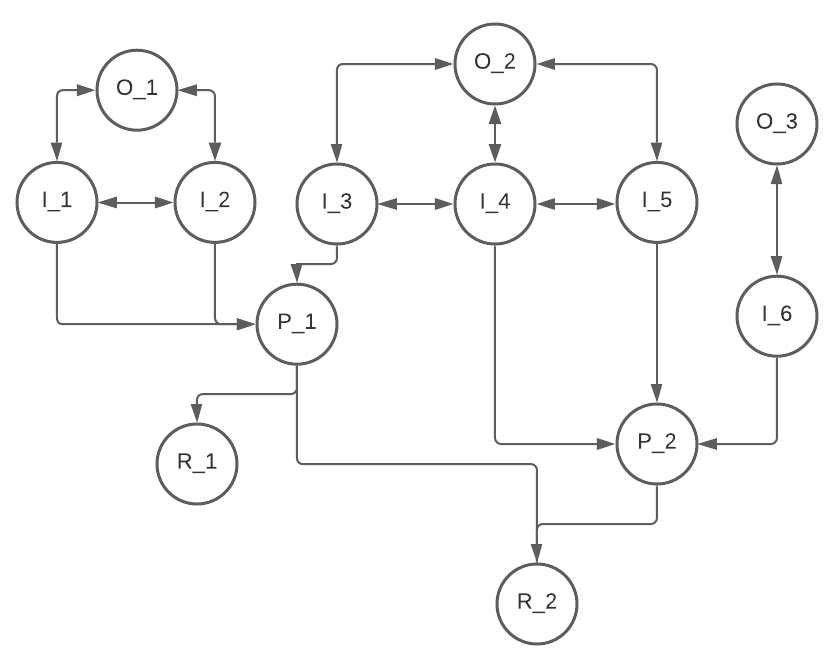
\includegraphics[scale=0.5]{images/descendants.png}
	\caption{Example of an Object Descendant Graph}
	\label{fig:descendant-graph}
\end{figure}


\subsection{Object Lineage Graph}
\textbf{Description -}\\
\noindent\textbf{Context -}\\
\noindent\textbf{Strengths}\\
\noindent\textbf{Limitations}\\
\noindent\textbf{Visual Example}
\begin{figure}[h]
	\centering
	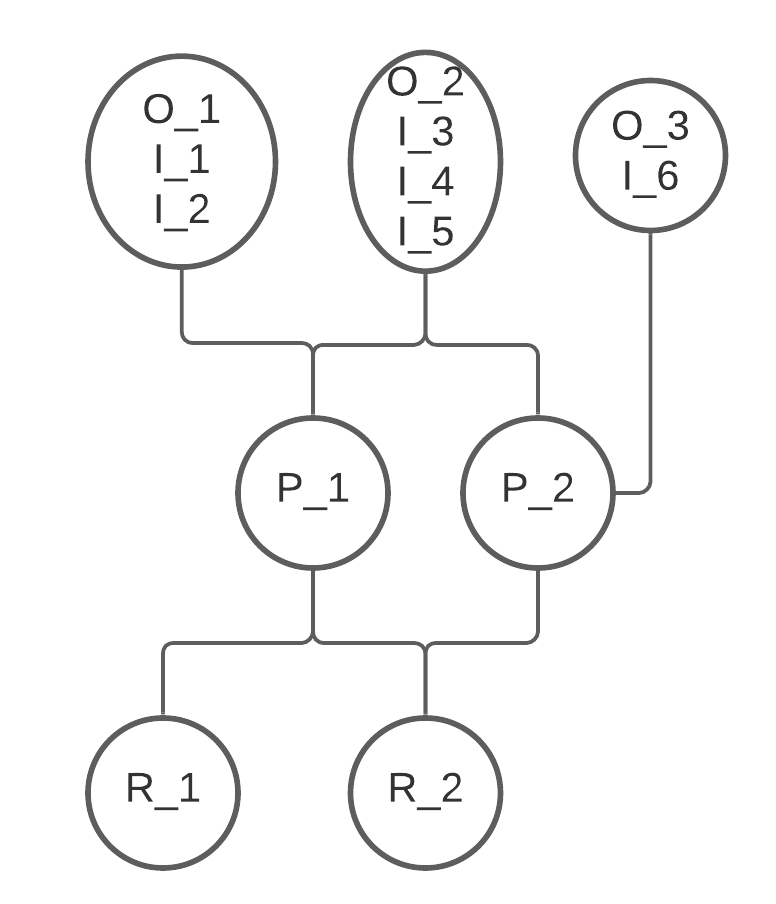
\includegraphics[scale=0.8]{images/lineage.png}
	\caption{Example of a Lineage Graph}
	\label{fig:lineage}
\end{figure}

\subsection{Event-Based}
\section{Object Based Features}
\subsection{Point wise Features}
This section includes features that are related to single objects. This means that each object produces its own vector which can be used for further computation.
\subsubsection{Activity Existence}
\begin{center}
	\begin{tabular}{| p{3cm} p{7cm} |}
		\hline
		\textbf{Property} & \textbf{Value}\\
		\hline
		User Input & None\\
		Structure Input & None\\
		Output & OHE of activity names per object\\
		Function Name & add\_activity\_existence\\
		\hline
	\end{tabular}
\end{center}

\textbf{Context -} The goal of this feature is to get a representation of which activities each object participates in. This gives an overall view of how an object participates does action in a log.\\

\subsubsection{Object Lifetime}
\begin{center}
	\begin{tabular}{| p{3cm} p{7cm} |}
		\hline
		\textbf{Property} & \textbf{Value}\\
		\hline
		User Input & None\\
		Structure Input & None\\
		Output & uint64 seconds an object lived\\
		Function Name & add\_object\_lifetime\\
		\hline
	\end{tabular}
\end{center}

\textbf{Context -} The goal of this feature is to understand how long an object was interacting in the system.\\

\subsubsection{Object Unit Set Ratio}
\begin{center}
	\begin{tabular}{| p{3cm} p{7cm} |}
		\hline
		\textbf{Property} & \textbf{Value}\\
		\hline
		User Input & None\\
		Structure Input & None\\
		Output & float64 [0,1] ratio being a unit set in type\\
		Function Name & add\_obj\_unit\_set\_ratio\\
		\hline
	\end{tabular}
\end{center}

\textbf{Context -} The goal of this feature is to understand what type of object it is. Whether it operates alone as a type (eg. Orders) or with many other of the same type (eg. items) throughout all events it takes part in.
\\

\subsubsection{Average number of other objects in Events} 
\begin{center}
	\begin{tabular}{| p{3cm} p{7cm} |}
		\hline
		\textbf{Property} & \textbf{Value}\\
		\hline
		User Input & None\\
		Structure Input & None\\
		Output & float64 avg object interactions per event\\
		Function Name & add\_avg\_obj\_event\_interaction\\
		\hline
	\end{tabular}
\end{center}

\textbf{Context -} The goal of this feature is to understand how social the object is with any other type of object while executing events. 
\\
\subsubsection{Unique Neighbor Count}
\begin{center}
	\begin{tabular}{| p{3cm} p{7cm} |}
		\hline
		\textbf{Property} & \textbf{Value}\\
		\hline
		User Input & None\\
		Structure Input & Object Graph\\
		Output & uint64 number of neighboring objects\\
		Function Name & add\_unique\_neighbor\_count\\
		\hline
	\end{tabular}
\end{center}

\textbf{Context -} The goal of this feature is to understand with how many objects in total the target object is working with.
\\

\textbf{Visual example}
\begin{figure}[h]
	\centering
	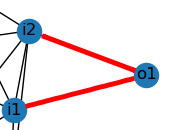
\includegraphics[scale=0.5]{images/obj-unc.png}
	\caption{o1 has two unique neighbors. i1 and i2.}
	\label{fig:obj-unc}
\end{figure}

\subsubsection{Object Type Interaction Count}
\begin{center}
	\begin{tabular}{| p{3cm} p{7cm} |}
		\hline
		\textbf{Property} & \textbf{Value}\\
		\hline
		User Input & Object Type (Default: All)\\
		Structure Input & Object Graph\\
		Output & uint64 number for each input object type\\
		Function Name & TBA\\
		\hline
	\end{tabular}
\end{center}

\textbf{Context -} The goal of this feature is to quantize to what type of objects the target object is interacting with in all events.
\\

\textbf{Visual example}
\begin{figure}[h]
	\centering
	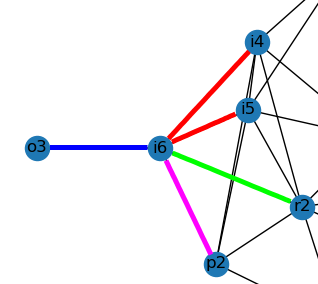
\includegraphics[scale=0.5]{images/obj-tic.png}
	\caption{Object i6 has 5 neighbors. There is 1 of order, package, route and 2 are of type item}
	\label{fig:obj-tic}
\end{figure}

\subsubsection{starting or ending object}
\begin{center}
	\begin{tabular}{| p{3cm} p{7cm} |}
		\hline
		\textbf{Property} & \textbf{Value}\\
		\hline
		User Input & None\\
		Structure Input & Object Lineage Graph\\
		Output & bool for each column\\
		Function Name & TBA\\
		\hline
	\end{tabular}
\end{center}

\textbf{Context -} The goal of this feature is to see whether the target object is a root or a leaf object. These bool values could add understanding to positioning in the lifecycle of a collection of objects.
\\

\textbf{Visual example}
need to update graph

\subsubsection{Direct Object Descendants / Ascendants number}
\begin{center}
	\begin{tabular}{| p{3cm} p{7cm} |}
		\hline
		\textbf{Property} & \textbf{Value}\\
		\hline
		User Input & None\\
		Structure Input & Object Lineage Graph\\
		Output & uint64 number for each direction\\
		Function Name & TBA\\
		\hline
	\end{tabular}
\end{center}

\textbf{Context -} The goal of this feature is to understand from where the object originates and where the object leads to.
\\

\textbf{Visual example}
\begin{figure}[h]
	\centering
	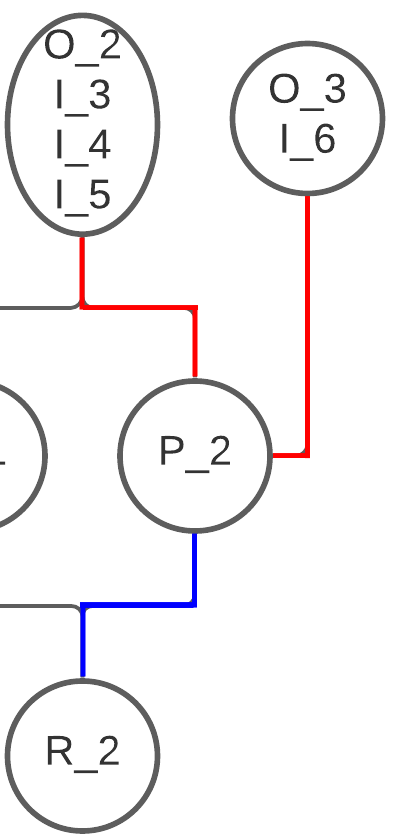
\includegraphics[scale=0.2]{images/obj-dda.png}
	\caption{P\_2 has two direct ascendants and one direct descendant}
	\label{fig:obj-dda}
\end{figure}

\subsubsection{Lineage Level with total height of lineage}
\begin{center}
	\begin{tabular}{| p{3cm} p{7cm} |}
		\hline
		\textbf{Property} & \textbf{Value}\\
		\hline
		User Input & None\\
		Structure Input & Object Lineage Graph\\
		Output & uint64 numbers for level and total height\\
		Function Name & TBA\\
		\hline
	\end{tabular}
\end{center}

\textbf{Context -} The goal of this feature is to understand how far through the object chain, the target object is first witnessed.
\\

\textbf{Visual example}

\begin{figure}[h]
	\centering
	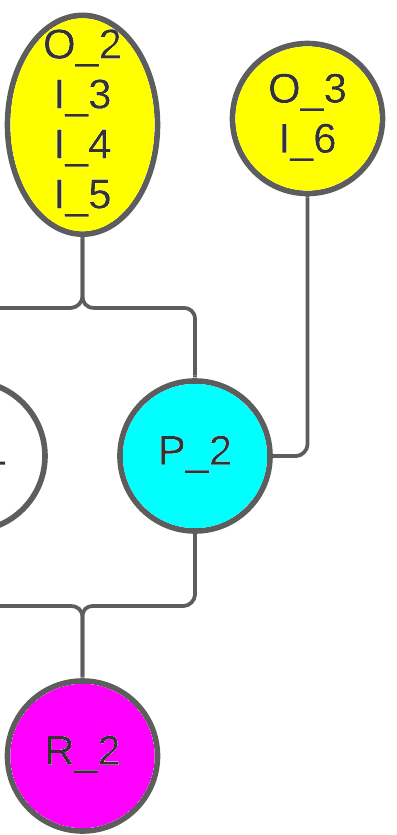
\includegraphics[scale=0.2]{images/obj-lvl.png}
	\caption{P\_2 only has direct ancestors and neighbors. Therefore P\_2 sits at level 2 out of 3}
	\label{fig:obj-lvl}
\end{figure}

\subsubsection{Object Wait time for specific event}
\begin{center}
	\begin{tabular}{| p{3cm} p{7cm} |}
		\hline
		\textbf{Property} & \textbf{Value}\\
		\hline
		User Input & Source Activity Name AND Target activity name\\
		Structure Input & None\\
		Output & uint64 time in seconds\\
		Function Name & TBA\\
		\hline
	\end{tabular}
\end{center}

\textbf{Context -} The goal of this feature is to differentiate between items and see how long an object has to wait in order for the next step to initiate. Eg. From Figure \ref{fig:log}: If pick\_item is the source and pack\_items is the target, the time i1 has to wait for pack\_items to occur is far greater than i3's wait time.
\\

\textbf{Visual example}
\subsubsection{Object specific event directly follows}
\begin{center}
	\begin{tabular}{| p{3cm} p{7cm} |}
		\hline
		\textbf{Property} & \textbf{Value}\\
		\hline
		User Input & None\\
		Structure Input & None\\
		Output & uint64 for DF in the events (with frequency information)\\
		Function Name & TBA\\
		\hline
	\end{tabular}
\end{center}

\textbf{Context -} The goal of this feature is to differentiate between how objects live in the ocel log. Allows to separate objects with different behaviors for further analysis
\\

\subsection{Local Features}
\subsection{Global Features}
\section{Event Based Features}
\subsection{Point wise Features}

\subsubsection{Number of objects involved separated by object type}
\begin{center}
	\begin{tabular}{| p{3cm} p{7cm} |}
		\hline
		\textbf{Property} & \textbf{Value}\\
		\hline
		User Input & None\\
		Structure Input & None\\
		Output & uint64 for each object type in log\\
		Function Name & TBA\\
		\hline
	\end{tabular}
\end{center}

\textbf{Context -} The goal of this feature is to assign the different types of objects in a numerical way.
\\

\subsubsection{Number of objects created by event per object type}
\begin{center}
	\begin{tabular}{| p{3cm} p{7cm} |}
		\hline
		\textbf{Property} & \textbf{Value}\\
		\hline
		User Input & None\\
		Structure Input & None\\
		Output & uint64 number for each object type\\
		Function Name & TBA\\
		\hline
	\end{tabular}
\end{center}

\textbf{Context -} The goal of this feature is to differentiate between objects that have already been seen in the log and objects that appear for the first time in the event.
\\

\subsubsection{Activity of Event}
\begin{center}
	\begin{tabular}{| p{3cm} p{7cm} |}
		\hline
		\textbf{Property} & \textbf{Value}\\
		\hline
		User Input & None\\
		Structure Input & None\\
		Output & OHE of activity names\\
		Function Name & TBA\\
		\hline
	\end{tabular}
\end{center}

\textbf{Context -} The goal of this feature is to assign the activity name in a numerical way.
\\

\subsection{Local Features}
\subsection{Global Features}

\subsubsection{Time Series: rate of change of number of events occurring in the same time window}
\begin{center}
	\begin{tabular}{| p{3cm} p{7cm} |}
		\hline
		\textbf{Property} & \textbf{Value}\\
		\hline
		User Input & time window size\\
		Structure Input & None\\
		Output & float64 for each timewindow\\
		Function Name & TBA\\
		\hline
	\end{tabular}
\end{center}

\textbf{Context -} The goal of this feature is to gather information about how active the OCEL log is.
\\

\textbf{Visual Example}
TODO

\end{document}